\documentclass[12pt]{article}
\usepackage{setspace}
\usepackage[utf8]{inputenc}
\usepackage{graphicx}
\graphicspath{{img/}}
\usepackage{multicol}
\usepackage{hyperref}
\usepackage[export]{adjustbox}
\usepackage{subfig}
\usepackage{imakeidx}
\makeindex[columns=1, intoc]
\usepackage{amsmath}
\usepackage{indentfirst}

\title{Computational Cognition and Deep Learning}
\author{Andy Malinsky \\
Mentor: Dr. Katherine Moore}

\date{16 April 2019}

\begin{document}
\maketitle
\doublespacing
\begin{abstract}
    This paper surveys the current states of computational cognitive neuroscience and deep learning, focusing on three intersecting areas of active research. Discussed are the areas of vision, reinforcement learning, and natural language understanding. Each area involves the use of cognitive models known as deep artificial neural networks. Different types of these cognitive architectures are utilized for domain specific tasks, such as object recognition, game mastering, or language translation. Although the present successes of deep learning techniques represent a major breakthrough for data science, the prospect of achieving artificial general intelligence is yet to be determined. Solving the problem of intelligence, both biological and artificial, may be one of the biggest challenges in human history. This is why computational cognitive neuroscientists and deep learning researchers should combine their efforts to make progress in realizing this dream. 
\end{abstract}
\newpage
\tableofcontents
\newpage

\section{Introduction}
The fields of computational cognitive neuroscience and artificial intelligence have a particular goal in common, to understand the composition of intelligent cognition. One of the main underlying cognitive phenomena at the heart of intelligence research is the process of learning. Through cognitive modeling, neuroscientists are able to test their theories by trying to computationally emulate certain brain functions and cognitive processes. Artificial intelligence researchers, now more than ever, are implementing similar biologically inspired algorithms within a subfield of machine learning known as deep learning. Systems referred to as artificial neural networks are the focus of this subfield and are also techniques used in cognitive modeling. These architectures are designed to behave similarly to biological neural networks found in the brain. Breakthroughs in industry ranging from self-driving cars, mastering games through self-play, image classification, and language translation show just how powerful deep learning can be. In this paper, we discuss three active areas of research pertaining to both cognitive neuroscientists and deep learning researchers, including vision, reinforcement learning, and language understanding. Each of these areas requires some form of human-level understanding, which is still a leading problem in intelligence research. The proposed step forward in solving intelligence is to further merge cognitive neuroscience and deep learning research. New deep learning architectures may be utilized by cognitive neuroscientists and new computational models of cognition may be utilized by deep learning researchers. Artificial general intelligence, or a human-grade intelligent machine, is the ultimate goal of artificial intelligence research. Given our limited knowledge of the human brain, however, this notion may seem out of reach. But, with a focused attention on solving the ultimate problem of intelligence, we can hope to gain the potential to solve the world’s hardest problems.

\subsection{Intelligence Science}
One of the biggest fundamental mysteries of our universe is how the brain works. Current challenges in our understanding involve the underlying principles behind how the brain processes sensory input information up to thoughts then up to actions \cite{c11}. Let us define the term intelligence as human-level reasoning from these principles. A field of research coined Intelligence Science \cite{c1} is focused on understanding how the mind works by framing this research problem as the study of intelligence itself. This promotes more collaboration between cognitive neuroscientists and artificial intelligence researchers, as both groups share the same goal of understanding intelligence.

\subsection{Learning in the Brain}
To understand what we know so far about learning in the brain, it is important to have a general understanding of what neurons are and how they operate. The region of the brain known as the neocortex, a region where most of our cognitive thought takes place, houses around 20 billion neurons \cite{c3}. Each neuron is interconnected with roughly 10,000 others. Communication between neurons happens through synapses, or connection points, by means of electrical signals. Incoming signals carry synaptic weights, so depending on these weights the receiving neuron will either activate and send an output signal or not. Changes in synaptic weights, otherwise referred to as synaptic plasticity, as a function of local neural activity patterns between sending and receiving neurons is our fundamental understanding of how learning works in the brain. Everything that we learn is essentially different patterns of synaptic weights.

\subsection{Computational Cognitive Neuroscience}
Computational cognitive neuroscience involves the use of computer models as a means of understanding cognitive functions, which is a process known as cognitive modeling. This means that the methods employed are experimental interpretations based off of theories of certain brain functions. Deep learning involves the connectionist approach to cognitive modelling \cite{c5}, which entails large interconnected networks of simple numerical processors running in parallel. A popular type of connectionist model used in both computational cognitive neuroscience and in deep learning is artificial neural networks.

\subsection{Deep Learning}
Deep learning is a subfield of Machine Learning, which is a subfield of Artificial Intelligence (AI). Deep learning focuses on the use of deep neural networks to solve problems involving data. Artificial neural networks were designed to operate similarly to the biological neural networks found in the brain, as in continuously updating weights to ultimately “learn” from data. 
\subsubsection{Deep Artificial Neural Networks}
A neural network is said to be ``deep'' if it is comprised of multiple layers. A typical model has an input layer, many hidden layers, and an output layer. Each layer is made up of “neurons,” or nodes, and each node in a given layer is connected to each node in an adjacent layer with a given weight. These weights can then be adjusted based on a variation of the stochastic gradient descent model, for example, in order to minimize error in generated output values. Neuron activations are forward-and-back propagated through the layers of the network and the weights are updated accordingly. After the network goes through this training process, it should be able to take new input and output expected results with an ideally high accuracy. This is the fundamental way deep neural networks function, along with the foundational backpropagation algorithm.
\begin{figure}[ht!] %!t
\centering
\hspace*{0cm} 
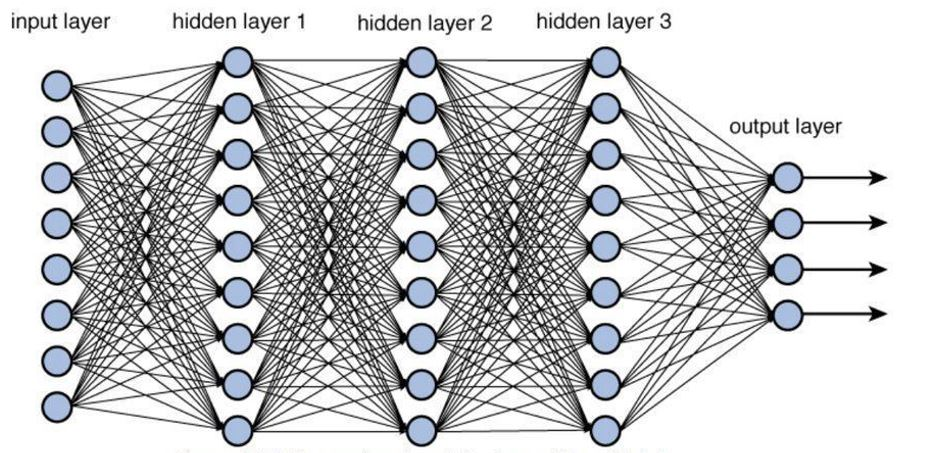
\includegraphics[height=2.5in]{deepNet.JPG}
\caption{This is a common graphical representation of a deep neural network model \cite{c16}.}
\label{deep_neural_net__example}
\end{figure} \\

\subsubsection{Biological Plausibility of the Backpropagation Algorithm}
The backpropagation algorithm has become a common tool for training deep neural networks \cite{c8}. The training process described earlier involves the use of this algorithm to adjust the weights of the network.
\begin{equation}\nonumber
\frac{\partial E}{\partial y_{i}} =\sum\limits _{j}\frac{\partial E}{\partial x_{j}}\frac{\partial x_{j}}{\partial y_{i}} =\sum\limits _{j}\frac{\partial E}{\partial x_{j}} w_{ij}
\end{equation} 

The mathematical equation above is the fourth part of the backpropagation algorithm, which computes how fast the error changes as the activity of a unit in the previous layer is changed \cite{c8}. The error derivatives are computed, where \emph{E} is the error, \emph{w$_{ij}$} is the weight of the connection between the \emph{i}th and \emph{j}th unit, and \emph{x$_j$} is the total weighted input. This equation is essentially just a part of what the neural network actually looks like, a series of mathematical computations. This idealized formulation has been the center of debate in the deep learning community, as the true method of learning in the human brain is yet to be discovered. Neural networks and the backpropagation algorithm were originally designed from the simplest understanding of changes in synaptic weights between neurons. A path toward more unsupervised approaches seem to be in order as the backpropagation model requires a ``teacher'' that can feed it labelled data. On the other hand, humans are capable of learning without a ``teacher'' when it comes to general problem-solving and critical thinking. Little is still known about the actual biological learning procedures found in the brain. Therefore, many believe that more biologically inspired deep learning algorithms have the potential to solve the biggest challenge in AI, artificial general intelligence (AGI).

\subsection{Artificial General Intelligence}
The goal of AGI is to create software or hardware systems with general intelligence comparable to or greater than that of a human \cite{c2}. AI company DeepMind developed an algorithm involving neural networks called AlphaZero that was able to master the 2,000-year-old game of Go in the space of a few days \cite{c4}. Computer programs have the ability to perform amounts of computations that would take humans hundreds or even thousands of years. The end goal is to apply this same level of computational analysis to optimize problems or find solutions in various domains such as healthcare, environment, finance, and society resource management. AI could uncover patterns in overwhelmingly complex datasets and suggest promising ideas and strategies \cite{c12}. To move the field forward, a unifying theory of intelligence would be most ideal, as it would apply to both neuroscience and AI research. A potential path toward this goal is to focus on the three key areas of vision, reinforcement learning, and natural language understanding, and developing more closely biologically inspired algorithms. Discussed in the following sections for each research area are the cognitive models and processes involved, along with some industry use cases.  

\section{Vision}
\subsection{From Eye to Brain}
Vision plays a crucial part in how we perceive and understand the world. The brain divides a continuous pattern of light into discrete objects and surfaces and translates the two-dimensional retinal image into a three-dimensional interactive model of the environment \cite{c6}. The main visual pathway in the brain is known as the primary visual cortex. Neurons in this brain region encode sensory input in terms of edges, or transitions of illumination, to begin developing a mental representation of the perceived natural physical image \cite{c3}. This cognitive process involves the three stages of perception, recognition, and action \cite{c9}. Perception is the sensory experience obtained from consciously translating an input image into a form of acknowledgement that an object has been \emph{perceived}. Recognition is our way of categorically identifying what we see. These categories may be developed through prior knowledge or experiences as they help shape our individual understanding. Then, action takes place in terms of activity in our motor systems. Depending on the stimulus being perceived, a resultant behavior is expected. This is a cognitive process that continuously runs during average daily activity, which makes it a process worth investigating as a contributing factor to understanding intelligence.  

\subsection{Computer Vision}
Common cognitive models used for object recognition tasks are known as convolutional neural networks. Inspired by the biological eye, the neural net scans the input image pixel by pixel, extracting features of the given objects. 
For example, if the task is to distinguish between a cat and dog, it can look for features such as “floppy” or “pointy” ears, “dog snout”, or “fur” \cite{c14}. Techniques such as feature visualization allow for a \emph{semantic dictionary} of how the network understands the input image as a whole. It would need to go through a training processes first in order to identify each feature representation.
\newpage
\begin{figure}[ht!]
  \centering
  \begin{minipage}[b]{0.4\textwidth}
    
\includegraphics[width=\textwidth]{animals.JPG}
    \caption{}
    \label{fig:animals}
  \end{minipage}
  \hfill
  \begin{minipage}[b]{0.4\textwidth}
    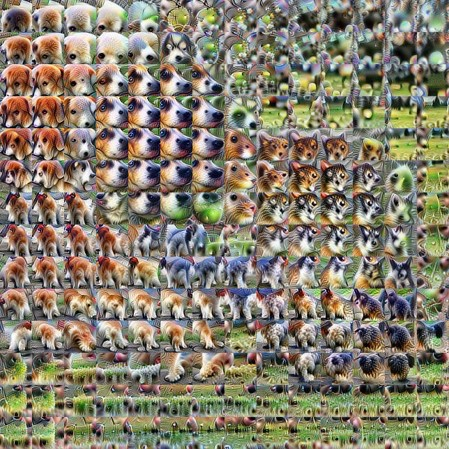
\includegraphics[width=\textwidth]{feature_visualization.JPG}
    \caption{}
    \label{fig:featureMap}
  \end{minipage}
\end{figure}

Depicted in Figure \ref{fig:animals} is a standard input image of two dominant objects each with representative features. This results in a feature visualization map, or a semantic dictionary of detected features as seen in Figure \ref{fig:featureMap} \cite{c14}.

\subsection{Limitations of Convolutional Neural Networks}
Convolutional neural networks have a great impact in emerging technologies such as self-driving cars and facial recognition, but deep learning for computer vision still has limitations. Training neural networks requires a large amount of labelled data. A network has to learn what “floppy ears” are before it can recognize them in an image. Also, bias in the lack of realistic examples such as varying viewpoints results in worse scene understanding and lower accuracies for object recognition. If the majority of training examples are similar to a particular angle, it may have a harder time recognizing an object in a new image that is from a completely different viewpoint \cite{c13}. Better methods for overall scene understanding and general contextualization is a current challenge. Therefore, current models still have room for improvement.

\section{Reinforcement Learning}
\subsection{Procedural Learning and Classical Conditioning}
Responses we get from external stimuli affect our behavior. The brain region responsible for learning from reward and punishment signals is known as the basal ganglia \cite{c3}. The actions we take are directly influenced by this specialized area, which results in a form of learning called reinforcement learning. Dopamine neurons activate when a reward is delivered which results in the conditioning of the brain to expect a reward upon taking a given action. This topic of conditioning is one that arises under procedural learning, with the category of associative learning \cite{c7}. This type of learning deals with procedural memories, in that a given sensory input generates a given motor or sensory output. These reactions can be learned, or conditioned, along reflex path ways in the brain. Classical conditioning is a type of associative learning and involves learning an association from two different stimuli to the same individual response \cite{c7, c18}. As seen in the famous experiment from Russian physiologist Ivan Pavlov, dogs were conditioned to salivate upon hearing a certain sound. The figure below illustrates the conditioning process.
\newpage

\begin{figure}[ht!] %!t
\centering
\hspace*{-0.3cm} 
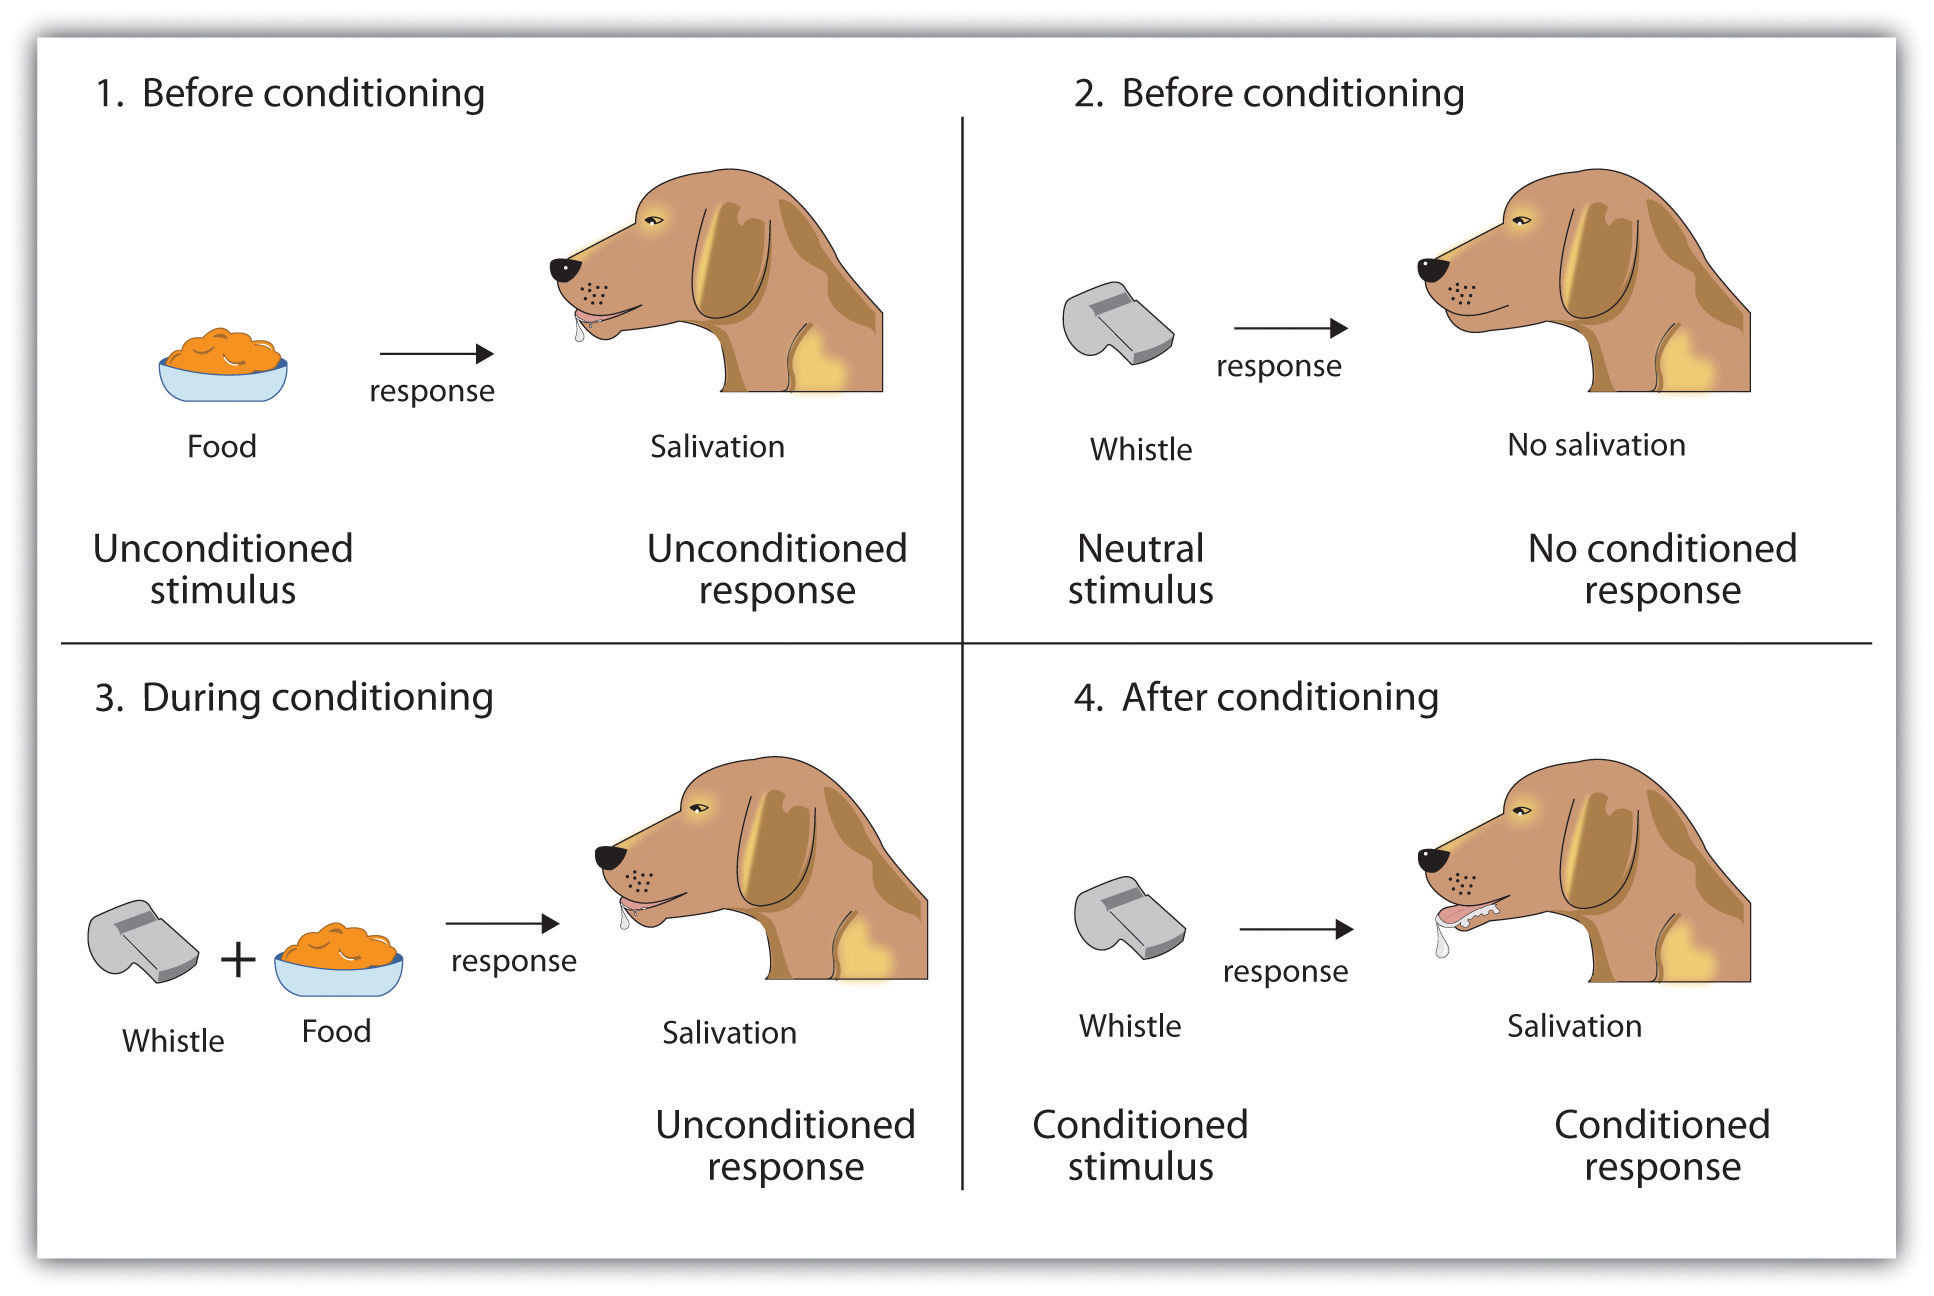
\includegraphics[height=3.5in]{conditioning.JPG}
\caption{An example of classical conditioning \cite{c18}.}
\label{conditioning}
\end{figure}

The dog in the experiment learns a new association between the presence of the food and an auditory stimulus. This is essentially a form of reinforcement learning taking place in that the dog will predict food to arrive upon hearing the same sound, thus resulting in the expected response. Conditioning and reinforcement learning processes are evolutionarily beneficial \cite{c18}, because it allows for the development of new associations between particular stimuli and good or bad events. Cognitive reinforcement learning provided the inspiration for cutting-edge computational models employed for deep learning. 

\subsection{Deep Reinforcement Learning}
DeepMind’s program AlphaZero also learned to master the game of Chess through the process of reinforcement learning. Using a deep neural network architecture comprising of many layers, it learns by self-play. Based on results from wins, losses, and draws, it adjusts the network’s parameters to make it more likely to choose better moves in the future \cite{c4}.

The reason why AlphaZero is unique is because it is general purpose. It is able to learn any two-player perfect information game given just the set rules to follow. This is a big step forward toward AGI, but a potential route for further research is to implement transfer learning. For example, a person who knows how to play the guitar may be able to pick up the piano faster than someone with no musical background \cite{c15}. Learning from reinforcement and then transferring gained knowledge to new tasks is something that the human brain is very good at, so perhaps AI research should be paying more attention to that neuroscience for inspiration.

\section{Natural Language Understanding}
\subsection{Semantic Meaning and Memory}
Human language is a unique form of communication from our non-human counterparts. People are able to understand each other based on individual systems of semantic representations, or relationships between words and symbols to their meaning in reality. This is the idea behind a dominant notion of amodal, or abstract memory \cite{c6}. This cognitive process is displayed in the hub-and-spoke model as depicted in the figure below.\\
\begin{figure}[ht!] %!t
\centering
\hspace*{-0.3cm} 
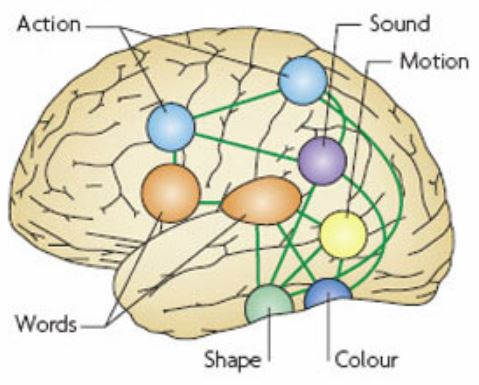
\includegraphics[height=2.5in]{semanticBrain.JPG}
\caption{The hub-and-spoke model is a hybrid model of semantic memory, containing both amodal and grounded representations in sensory and motor systems \cite{c6, c17}. Processes similar to that of mental imagery take place, which can make sense intuitively. People essentially translate generated mental images and associations into representative words. These words are ingrained through a training or learning process, as people develop those connections, or associations.}
\label{semantic_brain}
\end{figure}

For example, consider the word ``elephant'' and one may recall associated properties such as long trunk, animal, big ears, gray skin, etc... In this sense, the linguistical symbol grounding problem arises, in that there must be a way to define words without the use of other words. Concepts such as embodied cognition offer grounded associations, such as actions of the motor system or perceptual experiences in relation to understanding communicative words. Current language modelling networks in industry may take slightly different approaches.

\subsection{Natural Language Processing}
Computational algorithms that automatically analyze and represent human language fall under the category of Natural Language Processing (NLP). One deep learning approach to NLP is the use of recurrent neural networks. This type of model uses a computational structure known as ``Long Short-Term Memory'' which is able to process through sequences of data with a temporal internal state memory \cite{c19}. This is An example that utilizes this technology is Google Translate \cite{c10}. Google Translate is an example of Neural Machine Translation, in which it encodes the source language and decodes to the target language. It uses sequence to sequence modelling to summarize the source sentence in the translated version. In addition, when it comes to reading written language, we are able to recognize words with spatial invariance, so we can distinguish words even if their appearance varies. This is clearly evident in the figure below:
\newpage
\begin{figure}[ht!] %!t
\centering
\hspace*{-0.3cm} 
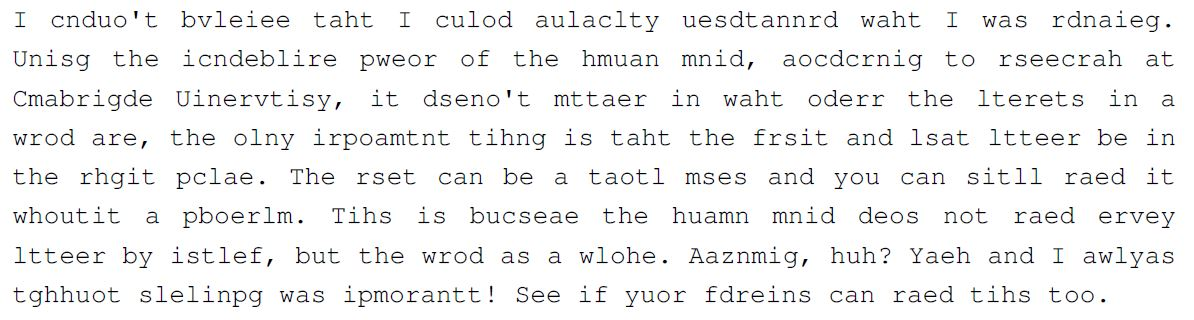
\includegraphics[height=1.5in]{spatialInv.JPG}
\caption{This is an example of spatial invariance found in reading text \cite{c3}.}
\label{spatial_invariance_example}
\end{figure}

Similar to computer vision tasks, language reading may also take the form of object recognition. Our brains went through a form of training process when first learning how to read. Connections are made between visually interpreted symbols to their corresponding sound and ultimately to their corresponding objective meaning. Spatial invariance in reading shows that when given a set of characters that form a word, as long as the first and last letter remain intact one can still recognize that given word by inferring known letters to be in their commmon positions. Studying this phenomena gives us insight into how the brain processes visual symbolic representations of words and ideas. 

Language modelling has seen great breakthroughs such as Google Translate, but there are still limitations. Semantic understanding is the direction for further research. Exactly how people acquire languages and develop higher-level semantic representations may provide insights into different functions of intelligence.

\section{Conclusion}
We are currently in a technological revolution that is rapidly developing. Computational cognitive neuroscience has set the foundation for deep learning as we have seen the power of artificial neural networks. Inspired by areas of human cognition, including vision, reinforcement learning, and natural language understanding, computational models have been developed in an effort to mimic the complexity of the human brain. However, there is still room for improvement as we have yet to fully solve the function of intelligence. Many say that we are far away from AGI, but with a stronger coordinated effort between neuroscientists and deep learning researchers, the world’s hardest problems may be solved sooner rather than later.

\begin{thebibliography}{50}

\bibitem{c1} Cassimatis, N. L. (2012). Artificial intelligence and cognitive modeling have the same problem. In Theoretical Foundations of Artificial General Intelligence (pp. 11-24). Atlantis Press, Paris.
\bibitem{c2} Goertzel, B. (2014). Artificial general intelligence: concept, state of the art, and future prospects. Journal of Artificial General Intelligence, 5(1), 1-48.
\bibitem{c3} O'Reilly, R. C., Munakata, Y., Frank, M. J., Hazy, T. E., and Contributors (2012). Computational Cognitive Neuroscience. Wiki Book, 1st Edition. URL: http:/ / ccnbook. colorado. edu
\bibitem{c4} Silver, D., Hubert, T., Schrittwieser, J., Antonoglou, I., Lai, M., Guez, A., ... \& Lillicrap, T. (2017). Mastering chess and shogi by self-play with a general reinforcement learning algorithm. arXiv preprint arXiv:1712.01815.
\bibitem{c5} Smolensky, P. (1987). Connectionist AI, symbolic AI, and the brain. Artificial Intelligence Review, 1(2), 95-109.
\bibitem{c6} Ward, Jamie. The Student’s Guide to Cognitive Neuroscience. 3rd ed., Psychology Press, 2015. Print.
\bibitem{c7} Bear, Mark F, et al. Neuroscience: exploring the brain. 3rd ed., Lippincott Williams \& Wilkins, 2007. Print.
\bibitem{c8} Polk, Thad A., and Seifert, Colleen M. Cognitive Modeling. Cambridge: The MIT Press, 2002. Print.
\bibitem{c9} Goldstein, E. Bruce. Sensation and Perception, Eight Edition. Wadsworth, Cengage Learning, 2010. Print.
\bibitem{c10} Le, James. 2018 Sep 3. Recurrent Neural Networks: The Powerhouse of Language Modeling [blog]. Towards Data Science. https://towardsdatascience.com/recurrent-neural-networks-the-powerhouse-of-language-modeling-d45acc50444f.
\bibitem{c11} Siegfried, Tom. 2017 July 25. There’s a long way to go in understanding the brain [blog]. ScienceNews. https://www.sciencenews.org/blog/context/neuroscience-understanding-brain
\bibitem{c12} AI and the world’s complex challenges. c2019. DeepMind Technologies Limited. https://deepmind.com/applied/deepmind-ethics-society/research/AI-worlds-complex-challenges/.
\bibitem{c13} Yuille, A. L., \& Liu, C. (2018). Deep Nets: What have they ever done for Vision?. arXiv preprint arXiv:1805.04025.
\bibitem{c14} Olah, C., Satyanarayan, A., Johnson, I., Carter, S., Schubert, L., Ye, K., \& Mordvintsev, A. (2018). The building blocks of interpretability. Distill, 3(3), e10.
\bibitem{c15} Weiss, K., \& Khoshgoftaar, T., \& Wang, D. (2016). A survey of Transfer Learning. Journal of Big Data. 3. DOI: 10.1186/s40537-016-0043-6.
\bibitem{c16} Parmar, Ravindra. 2018 Sep 11. Training Deep Neural Networks [blog]. Towards Data Science. https://towardsdatascience.com/training-deep-neural-networks-9fdb1964b964.
\bibitem{c17} Hickok, Greg. 2008 Jan 15. Adapted from Patterson et al., 2007. Accessed from http://www.talkingbrains.org/2008/01/semantics-and-brain-more-on-atl-as-hub.html.
\bibitem{c18} Stangor, Charles. 8.1 Learning by Association: Classical Conditioning. Introduction to Psychology, 1st Canadian Edition. https://opentextbc.ca/introductiontopsychology/chapter/7-1-learning-by-association-classical-conditioning/.
\bibitem{c19} Hochreiter, S., \& Schmidhuber, J. (1997). Long short-term memory. Neural computation, 9(8), 1735-1780.

\end{thebibliography}
\end{document}